\chapter{Espectrometría de masas y espectroscopia atómica}\label{ch:b2:mass-spec-atomic}

Los fuegos artificiales son rojos con sales de estroncio, verdes con sales de bario, amarillos con sodio: una llama convierte
los átomos en luz de colores que los identifican. Un espectrómetro de masas, de aspecto más modesto,
pesa moléculas una a una, las clasifica según sus isótopos y las rompe en fragmentos cuyas masas indican
cómo estaban construidas. Ambas técnicas responden a la pregunta ``¿qué hay en esta muestra, y cuánto?''
a partir de cantidades muy pequeñas, la primera para las moléculas, la segunda para los elementos.

\begin{omfigure}
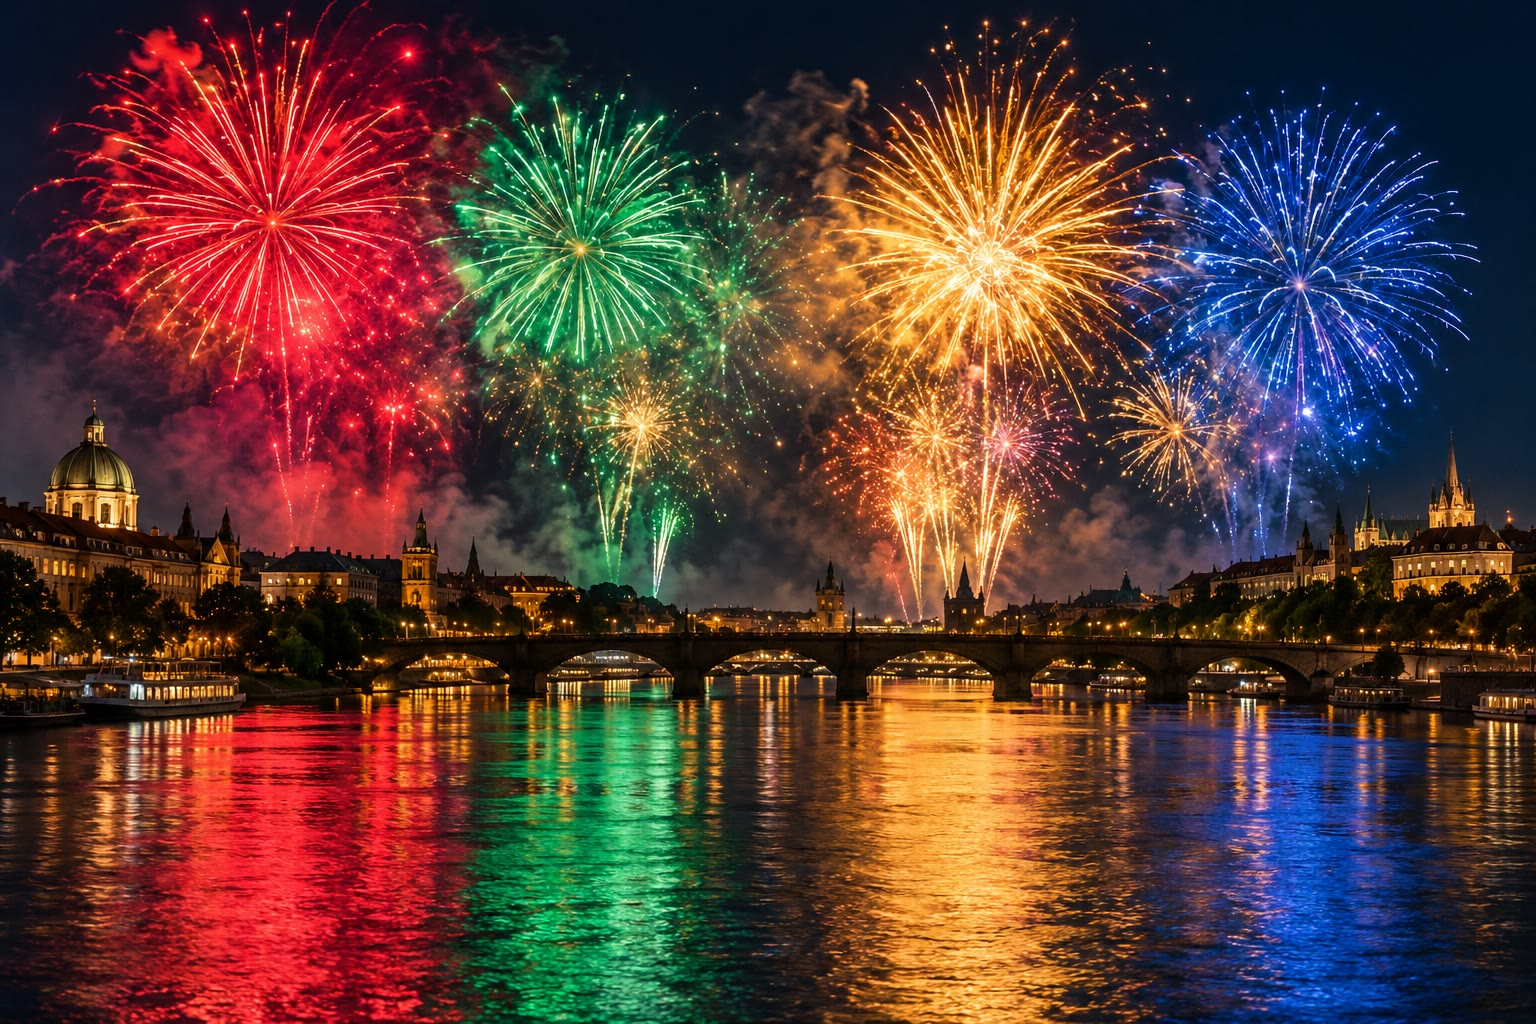
\includegraphics[width=0.58\linewidth]{images/book3/ai/b2-32-fireworks.jpg}

{\small Fuegos artificiales sobre un río (ilustración). El amarillo del sodio es la luz de sus átomos; los
rojos y verdes intensos proceden en gran parte de pequeñas moléculas de estroncio y de bario formadas en la llama.}
\end{omfigure}

\begin{recall}
El volumen escolar: los isótopos y sus abundancias. El volumen del primer año: niveles de energía y rayas
espectrales, absorbancia y ley de Beer--Lambert, carbocationes y radicales, grado de insaturación.
\Cref{ch:b2:chromatography}: la \omterm{def:b2:chromatography:techniques}{cromatografía de gases}, que a menudo alimenta un espectrómetro de masas.
\end{recall}

\section{El espectrómetro de masas}

\begin{definition}[Espectrometría de masas]\label{def:b2:mass-spec-atomic:spectrum}
La \emph{espectrometría de masas}\index{espectrometria de masas@espectrometría de masas} convierte las moléculas de una muestra en iones gaseosos,
separa los iones según su \emph{relación masa/carga}\index{relacion masa/carga@relación masa/carga} $m/z$
(la masa en unidades de masa atómica unificadas dividida por el número de cargas) y los cuenta. El
\emph{espectro de masas}\index{espectro de masas} representa la abundancia de los iones frente a $m/z$, normalmente como
intensidades relativas; su pico más intenso, al que se asigna el valor 100, es el \emph{pico base}\index{pico base}.
\end{definition}

Un espectrómetro tiene tres partes. La fuente produce los iones. En la ionización electrónica (IE), el vapor de la
muestra atraviesa un haz de electrones de \qty{70}{eV}, que arrancan un electrón a las moléculas y
las dejan con un exceso de energía, de modo que muchas se rompen. En la ionización por electrospray (ESI), una disolución se
pulveriza desde una aguja cargada; a medida que las gotitas se evaporan, las moléculas las abandonan llevando un protón adicional
(o un ion sodio), intactas: el método preferido para las moléculas grandes y frágiles. El analizador clasifica después
los iones, y un detector los cuenta.

\begin{omfigure}
\begin{tikzpicture}[x=1cm, y=1cm]
\draw[black!70, fill=omDef!10, rounded corners=2pt] (0,-0.6) rectangle (1.6,0.6);
\node[font=\small, align=center] at (0.8,0) {fuente\\de iones};
\draw[black!70] (2.0,-0.7) -- (2.0,0.7); \draw[black!70] (2.4,-0.7) -- (2.4,0.7);
\node[font=\footnotesize] at (2.2,1.0) {rejillas, $U$};
\draw[black!70] (2.6,-0.5) rectangle (8.4,0.5);
\node[font=\small] at (5.6,0.8) {tubo sin campo, longitud $L$};
\draw[black!70, fill=black!15] (8.5,-0.6) rectangle (8.8,0.6);
\node[font=\small, align=center] at (9.6,0) {detector};
\foreach \x/\c in {3.4/omThm, 4.6/omDef, 6.3/omMeth}{\fill[\c] (\x,0) circle (0.1);}
\draw[->, thick] (6.6,0) -- (7.4,0);
\node[font=\footnotesize, align=center] at (5.5,-0.85) {los iones ligeros se adelantan, los pesados se retrasan};
\end{tikzpicture}
\par\vspace{4pt}

{\small Un analizador de tiempo de vuelo (esquema). Los iones acelerados por la misma diferencia de potencial
$U$ salen con la misma energía cinética; en el tubo de vuelo los más ligeros viajan más deprisa y llegan antes al
detector.}
\end{omfigure}

\begin{proposition}[Tiempo de vuelo]\label{prop:b2:mass-spec-atomic:time-of-flight}
Un ion de masa $m$ y carga $ze$, acelerado desde el reposo por una diferencia de potencial $U$, atraviesa un
tubo libre de campo de longitud $L$ en
\begin{equation*}
t = L\sqrt{\frac{m}{2zeU}}:
\end{equation*}
el tiempo de vuelo crece como la raíz cuadrada de $m/z$.
\end{proposition}

\begin{proof}
La conservación de la energía en el campo acelerador da $\tfrac12mv^2 = zeU$, luego $v = \sqrt{2zeU/m}$, y
el tubo se recorre a velocidad constante: $t = L/v$.
\end{proof}

Otros analizadores clasifican los iones de otro modo: un cuadrupolo solo deja pasar los iones de una $m/z$ cada vez,
seleccionada mediante tensiones oscilantes en cuatro barras; un sector magnético curva los iones sobre círculos cuyo radio
depende de su cantidad de movimiento. En todos ellos solo se mide $m/z$; la mayoría de los iones producidos por IE llevan una sola
carga, de modo que $m/z$ es simplemente su masa.

\section{El ion molecular}

\begin{definition}[Ion molecular e iones fragmento]\label{def:b2:mass-spec-atomic:molecular-ion}
El \emph{ion molecular}\index{ion molecular} $\mathrm M^{+\bullet}$ es el catión radical que se forma cuando una
molécula pierde un electrón; su $m/z$ es la masa molar de la molécula formada por los isótopos más
abundantes. Un \emph{ion fragmento}\index{ion fragmento} procede del ion molecular por ruptura de
enlaces.
\end{definition}

El \omterm{def:b2:mass-spec-atomic:molecular-ion}{ion molecular} da la masa molecular, el primer dato sobre una sustancia desconocida. A veces es débil o
ausente en IE, cuando el \omterm{def:b2:mass-spec-atomic:molecular-ion}{ion molecular} se rompe con demasiada facilidad; el electrospray, que da $[\mathrm M +
\mathrm H]^+$ una unidad por encima, lo confirma entonces.

\begin{definition}[Regla del nitrógeno]\label{def:b2:mass-spec-atomic:nitrogen-rule}
La \emph{regla del nitrógeno}\index{regla del nitrogeno@regla del nitrógeno} afirma que una molécula tiene una masa nominal impar (la suma
de los números másicos de sus isótopos más abundantes) si y solo si contiene un número impar de átomos de
nitrógeno.
\end{definition}

\begin{proposition}[Validez de la regla del nitrógeno]\label{prop:b2:mass-spec-atomic:nitrogen-rule}
La \omterm{def:b2:mass-spec-atomic:nitrogen-rule}{regla del nitrógeno} se cumple para toda molécula sin electrones desapareados formada por C, H, N, O, S y los
halógenos.
\end{proposition}

\begin{proof}
Las masas nominales son pares para C (12), N (14), O (16) y S (32), e impares para H (1) y los halógenos (19,
35, 79, 127). Las valencias son pares para C, O y S, e impares para H, N y los halógenos. En una molécula
sin electrones desapareados, cada enlace usa una valencia de cada uno de sus dos átomos, de modo que la suma de todas las
valencias es par, y el número de átomos de valencia impar, $n_{\ce{H}} + n_{\ce{X}} + n_{\ce{N}}$, es
par. La paridad de la masa nominal es la de $n_{\ce{H}} + n_{\ce{X}}$, que es por tanto la de
$n_{\ce{N}}$.
\end{proof}

\begin{definition}[Perfil isotópico]\label{def:b2:mass-spec-atomic:isotope-pattern}
El \emph{perfil isotópico}\index{perfil isotopico@perfil isotópico} de un ion es el grupo de picos en $M$, $M+1$,
$M+2$, \dots\ producidos por las moléculas que contienen isótopos más pesados, con intensidades proporcionales a
las abundancias de esas formas isotópicas.
\end{definition}

\begin{proposition}[El pico $M+1$]\label{prop:b2:mass-spec-atomic:m-plus-one}
Para un ion con $n_C$ átomos de carbono y ningún otro elemento con un isótopo $+1$ significativo,
\begin{equation*}
\frac{I(M+1)}{I(M)} \approx n_C\,\frac{a_{13}}{a_{12}} \approx n_C \times 1.1~\%,
\end{equation*}
donde $a_{12} = 0.989$ y $a_{13} = 0.011$ son las fracciones molares de los dos isótopos del carbono.
% ledger: iso:C12, iso:C13
\end{proposition}

\begin{proof}
La probabilidad de que los $n_C$ carbonos sean todos \ce{^{12}C} es $a_{12}^{n_C}$; la de que exactamente uno sea
\ce{^{13}C} es $n_C\,a_{13}a_{12}^{n_C - 1}$ (ley binomial). La razón es $n_C\,a_{13}/a_{12}$, y las
demás contribuciones (dos \ce{^{13}C}, \ce{^2H}, \ce{^{15}N}) son menores en un factor del orden de
$a_{13}$ o inferior.
\end{proof}

\begin{proposition}[Cloro y bromo]\label{prop:b2:mass-spec-atomic:halogen-patterns}
Para un ion con $p$ átomos de cloro y $q$ de bromo, las intensidades de $M$, $M+2$, $M+4$, \dots\ son
los coeficientes del desarrollo de $(a_{35} + a_{37}x)^p(a_{79} + a_{81}x)^q$ en potencias de $x$, donde cada
potencia de $x$ representa 2 unidades de masa. Con $a_{35} = 0.758$, $a_{37} = 0.242$, $a_{79} = 0.5069$ y
$a_{81} = 0.4931$, un cloro da $M : M+2 \approx 3 : 1$, y un bromo, $\approx 1 : 1$.
% ledger: iso:Cl35, iso:Cl37, iso:Br79, iso:Br81
\end{proposition}

\begin{proof}
Cada átomo de halógeno es, de forma independiente, el isótopo ligero o el pesado, que añade 2 a la masa. La
probabilidad de un número dado $j$ de átomos pesados es el coeficiente de $x^j$ en el producto de un factor
por átomo, que es el desarrollo enunciado (la ley binomial, para cada elemento).
\end{proof}

\begin{omfigure}
\pgfplotsset{clu/.style={width=0.25\linewidth, height=3.3cm, ybar, bar width=5pt, ymin=0, ymax=118,
  xmin=-1.2, xmax=5.2, xtick={0,2,4}, xticklabels={$M$,$M\!+\!2$,$M\!+\!4$},
  tick label style={font=\tiny}, ytick=\empty, axis x line=bottom, axis y line=none,
  title style={font=\small, yshift=-4pt}, nodes near coords, nodes near coords style={font=\tiny},
  point meta=y, every node near coord/.append style={/pgf/number format/fixed, /pgf/number format/precision=0}}}
\begin{tikzpicture}
\begin{axis}[clu, title={Cl}]
\addplot[fill=omDef!55, draw=omDef, y filter/.expression={y==0 ? nan : y}] table[x=off, y=Cl] {figdata/out/bachelor-2-mass-spectra-a.dat};
\end{axis}
\end{tikzpicture}\hfill
\begin{tikzpicture}
\begin{axis}[clu, title={Cl$_2$}]
\addplot[fill=omDef!55, draw=omDef] table[x=off, y=Cl2] {figdata/out/bachelor-2-mass-spectra-a.dat};
\end{axis}
\end{tikzpicture}\hfill
\begin{tikzpicture}
\begin{axis}[clu, title={Br}]
\addplot[fill=omThm!45, draw=omThm, y filter/.expression={y==0 ? nan : y}] table[x=off, y=Br] {figdata/out/bachelor-2-mass-spectra-a.dat};
\end{axis}
\end{tikzpicture}\hfill
\begin{tikzpicture}
\begin{axis}[clu, title={Br$_2$}]
\addplot[fill=omThm!45, draw=omThm] table[x=off, y=Br2] {figdata/out/bachelor-2-mass-spectra-a.dat};
\end{axis}
\end{tikzpicture}\hfill
\begin{tikzpicture}
\begin{axis}[clu, title={ClBr}]
\addplot[fill=omMeth!45, draw=omMeth] table[x=off, y=ClBr] {figdata/out/bachelor-2-mass-spectra-a.dat};
\end{axis}
\end{tikzpicture}

{\small \omterm{def:b2:mass-spec-atomic:isotope-pattern}{Perfiles isotópicos} de iones que contienen cloro y bromo, calculados a partir de las abundancias
isotópicas (\cref{prop:b2:mass-spec-atomic:halogen-patterns}); el pico más intenso de cada grupo se
fija en 100. Los perfiles son huellas dactilares: 3 : 1 para un cloro, 1 : 1 para un bromo, 1 : 2 : 1
para dos bromos.}
% figdata: bachelor-2/mass-spectra.py part a
\end{omfigure}

\begin{definition}[Masa exacta]\label{def:b2:mass-spec-atomic:exact-mass}
La \emph{masa monoisotópica}\index{masa monoisotopica@masa monoisotópica} de un ion es la suma de las masas exactas de sus
isótopos más abundantes (\ce{^{12}C} = 12 exactamente, \ce{^1H} = 1.007825, \ce{^{16}O} = 15.994915,
\ce{^{14}N} = 14.003074 u). La \emph{espectrometría de masas de alta resolución}\index{espectrometria de masas de alta resolucion@espectrometría de masas de alta resolución}
mide $m/z$ con unas pocas milésimas de unidad o mejor, lo bastante para distinguir iones de la misma
masa nominal pero de fórmulas distintas.
% ledger: mass:C12, mass:H1, mass:O16, mass:N14
\end{definition}

\begin{proposition}[Poder de resolución]\label{prop:b2:mass-spec-atomic:resolving}
Dos iones de masas $m$ y $m + \Delta m$ quedan separados por un analizador de poder de resolución como mínimo
$R = m/\Delta m$. A la masa nominal 28, separar \ce{CO+} (27.9949) de \ce{N2+} (28.0061) requiere $R
\approx 2.5 \times 10^3$; separar \ce{N2+} de \ce{C2H4+} (28.0313), $R \approx 1.1 \times 10^3$.
\end{proposition}

\begin{proof}
El poder de resolución se define como $m/\Delta m$ para el menor $\Delta m$ que separa el analizador. Las
masas exactas se deducen de las masas isotópicas: $12 + 15.994915$, $2 \times 14.003074$, $24 + 4 \times
1.007825$; luego $28/(28.0061 - 27.9949) \approx 2.5 \times 10^3$ y $28/(28.0313 - 28.0061) \approx
1.1 \times 10^3$.
\end{proof}

\section{Fragmentación}

El \omterm{def:b2:mass-spec-atomic:molecular-ion}{ion molecular} producido por IE lleva mucha más energía de la que necesita cualquier enlace para romperse, y se rompe por
los caminos que dan los productos más estables: cationes estabilizados, moléculas neutras pequeñas y estables o
radicales. Los fragmentos se leen como pérdidas a partir de $M$ (15 para \ce{CH3}, 29 para \ce{C2H5} o \ce{CHO}, 18
para el agua, 28 para CO o el eteno) y como iones característicos.

\begin{definition}[Dos fragmentaciones]\label{def:b2:mass-spec-atomic:fragmentation}
En una \emph{ruptura $\alpha$}\index{ruptura alfa@ruptura $\alpha$}, se rompe un enlace del carbono contiguo a un
heteroátomo o a un carbonilo, lo que deja un catión estabilizado por el par no enlazante del heteroátomo (un \omterm{def:b2:aromatic-substitution:friedel-crafts}{ion
acilio} $\mathrm{R{-}C{\equiv}O^+}$ para una cetona, un ion iminio para una amina). La \emph{transposición de
McLafferty}\index{transposicion de McLafferty@transposición de McLafferty} de un compuesto carbonílico transfiere un hidrógeno del
carbono $\gamma$ al oxígeno carbonílico y rompe el enlace $\alpha$--$\beta$, liberando un alqueno y un
catión radical \omterm{def:b2:enolates-aldol:tautomerism}{enol}.
\end{definition}

\begin{omfigure}
\begin{tikzpicture}
\begin{axis}[width=0.48\linewidth, height=4.6cm, xmin=10, xmax=80, ymin=0, ymax=118,
  xlabel={$m/z$}, ylabel={intensidad relativa}, label style={font=\small}, tick label style={font=\scriptsize},
  title={\small butan-2-ona}, ycomb, xtick={15,29,43,57,72}]
\addplot[omDef, thick] table[x=mz, y=I] {figdata/out/bachelor-2-mass-spectra-b.dat};
\node[font=\tiny, anchor=south] at (axis cs:43,100) {43};
\node[font=\tiny, anchor=south] at (axis cs:72,25) {72};
\node[font=\tiny, anchor=south] at (axis cs:57,8) {57};
\node[font=\tiny, anchor=south] at (axis cs:29,17) {29};
\end{axis}
\end{tikzpicture}\hfill
\begin{tikzpicture}
\begin{axis}[width=0.48\linewidth, height=4.6cm, xmin=10, xmax=140, ymin=0, ymax=118,
  xlabel={$m/z$}, ylabel={intensidad relativa}, label style={font=\small}, tick label style={font=\scriptsize},
  title={\small 1-bromopropano}, ycomb, xtick={27,43,79,107,122}]
\addplot[omThm, thick] table[x=mz, y=I] {figdata/out/bachelor-2-mass-spectra-c.dat};
\node[font=\tiny, anchor=south] at (axis cs:43,100) {43};
\node[font=\tiny, anchor=south] at (axis cs:123,9) {122, 124};
\node[font=\tiny, anchor=south] at (axis cs:27,26) {27};
\node[font=\tiny, anchor=south east] at (axis cs:40.5,31) {41};
\end{axis}
\end{tikzpicture}

{\small Espectros de ionización electrónica (datos del NIST WebBook). Butan-2-ona: \omterm{def:b2:mass-spec-atomic:molecular-ion}{ion molecular} en 72;
las rupturas $\alpha$ dan los \omterm{def:b2:aromatic-substitution:friedel-crafts}{iones acilio} \ce{CH3CO+} (43, \omterm{def:b2:mass-spec-atomic:spectrum}{pico base}) y \ce{C2H5CO+} (57). 1-Bromopropano:
el \omterm{def:b2:mass-spec-atomic:molecular-ion}{ion molecular} es un par 1 : 1 en 122 y 124 (\ce{^{79}Br}, \ce{^{81}Br}); la pérdida del átomo de bromo
deja \ce{C3H7+} en 43, el \omterm{def:b2:mass-spec-atomic:spectrum}{pico base}.}
% figdata: bachelor-2/mass-spectra.py parts b, c
% ledger: ms:butanone, ms:bromopropane
\end{omfigure}

\begin{omfigure}
\setchemfig{atom sep=1.8em}
\schemestart
\chemfig{[:-30]\chemabove{O}{\scriptstyle +\bullet}?[a]=[:-90]C(-[:-150]H_3C)-[:-30]CH_2-[:30]CH_2-[:90]CH_2-[:150]H?[a,1,{dash pattern=on 1pt off 1.5pt}]}
\arrow{->}[,1.0]
\chemfig{CH_2=C(-[2]OH)-CH_3}\,$^{+\bullet}$
\+
\chemfig{CH_2=CH_2}
\schemestop
\par\vspace{6pt}

{\small La \omterm{def:b2:mass-spec-atomic:fragmentation}{transposición de McLafferty} de la pentan-2-ona, dibujada a través de su disposición cíclica de seis
eslabones: el hidrógeno del carbono $\gamma$ pasa al oxígeno, el enlace $\alpha$--$\beta$ se rompe,
sale eteno, y queda el catión radical \omterm{def:b2:enolates-aldol:tautomerism}{enol} de la propanona en $m/z$ 58.}
\end{omfigure}

\begin{proposition}[Condición de McLafferty]\label{prop:b2:mass-spec-atomic:mclafferty}
Una \omterm{def:b2:mass-spec-atomic:fragmentation}{transposición de McLafferty} requiere un hidrógeno en el carbono $\gamma$. Libera un alqueno y deja
un catión radical cuya masa tiene la paridad de la masa molecular (par para un compuesto sin
nitrógeno).
\end{proposition}

\begin{proof}[Argumento]
El hidrógeno se transfiere a través de una disposición cíclica de seis eslabones formada por el oxígeno, el carbono
carbonílico, los carbonos $\alpha$, $\beta$ y $\gamma$ y el propio hidrógeno: solo un hidrógeno $\gamma$
alcanza el oxígeno sin tensión. El ion formado conserva el grupo carbonilo, el carbono $\alpha$ y el
hidrógeno transferido; lo que sale es un alqueno, una molécula neutra de masa par, de modo que el ion conserva la
paridad de $M$, lo que lo distingue de los cationes de masa impar producidos por las rupturas simples.
\end{proof}

\begin{method}[Leer un espectro de masas]\label{met:b2:mass-spec-atomic:read-ms}
\begin{enumerate}
  \item Localícese el \omterm{def:b2:mass-spec-atomic:molecular-ion}{ion molecular} ($m/z$ más alta del grupo principal, con pérdidas razonables por debajo).
  \item Léase su \omterm{def:b2:mass-spec-atomic:isotope-pattern}{perfil isotópico}: Cl, Br, S; el pico $M+1$ da el número de carbonos.
  \item Aplíquese la \omterm{def:b2:mass-spec-atomic:nitrogen-rule}{regla del nitrógeno}; propónganse fórmulas y su grado de insaturación.
  \item Léanse las pérdidas a partir de $M$ y los iones característicos (43 \ce{CH3CO+} o \ce{C3H7+}, 77
        \ce{C6H5+}, 91 \ce{C7H7+}, 105 \ce{C6H5CO+}); búsquense iones de McLafferty de masa par.
  \item Propónganse estructuras; compruébese que todo pico importante queda explicado.
\end{enumerate}
\end{method}

\section{Espectroscopia atómica}

Los átomos no tienen vibraciones ni rotaciones; sus espectros son rayas finas, una por transición entre
niveles electrónicos, a longitudes de onda características del elemento. El amarillo de una llama de sodio es el
par de rayas a \qty{589.0}{nm} y \qty{589.6}{nm}; el carmesí del litio, una raya a \qty{670.8}{nm};
la raya más intensa de los átomos de estroncio está a \qty{460.7}{nm} y la de los iones de bario, a
\qty{455.4}{nm}, en el azul: los rojos y verdes de los fuegos artificiales proceden sobre todo de moléculas de estos
metales, no de sus átomos.
% ledger: asd:NaD2, asd:NaD1, asd:Li671, asd:Sr461, asd:Ba455

\begin{definition}[Espectrometrías atómicas]\label{def:b2:mass-spec-atomic:atomic}
En la \emph{espectrometría de emisión atómica}\index{espectrometria de emision atomica@espectrometría de emisión atómica} la muestra se atomiza y se
excita en una llama o un plasma, y se mide la intensidad de una raya de emisión del elemento. En la
\emph{espectrometría de absorción atómica}\index{espectrometria de absorcion atomica@espectrometría de absorción atómica} (EAA) la muestra se
atomiza en una llama o en un horno de grafito y se mide la absorbancia de los átomos en una raya de
resonancia, emitida por una \emph{lámpara de cátodo hueco}\index{lampara de catodo hueco@lámpara de cátodo hueco} cuyo cátodo está hecho del
propio elemento. En un \emph{plasma acoplado inductivamente}\index{plasma acoplado inductivamente} (ICP), el argón
calentado por un campo de radiofrecuencia a varios miles de kelvin atomiza e ioniza la muestra; el
plasma alimenta un espectrómetro de emisión (ICP-OES) o un espectrómetro de masas (ICP-MS).
\end{definition}

\begin{omfigure}
\begin{tikzpicture}[x=1cm, y=1cm, box/.style={draw=black!70, rounded corners=2pt, fill=white,
  font=\small, align=center, minimum height=0.8cm, inner sep=3pt}]
\node[box] (lamp) at (0,0) {lámpara de cátodo\\hueco (Cu)};
\shade[top color=omThm!60, bottom color=omThm!10] (2.6,-0.25) -- (3.3,-0.25) -- (3.15,0.75) -- (2.75,0.75) -- cycle;
\draw[black!70, fill=black!15] (2.4,-0.45) rectangle (3.5,-0.25);
\node[font=\footnotesize] at (2.95,-0.75) {llama (átomos)};
\node[box] (mono) at (6.1,0) {mono-\\cromador};
\node[box] (det) at (8.5,0) {detector};
\node[box] (data) at (10.8,0) {absorbancia};
\draw[->, thick, omDef] (lamp.east) -- (mono.west);
\draw[->, thick] (mono) -- (det); \draw[->, thick] (det) -- (data);
\node[font=\footnotesize, omDef] at (4.4,0.3) {$I_0 \to I$};
\end{tikzpicture}
\par\vspace{4pt}

{\small Un espectrómetro de absorción atómica (esquema). La lámpara emite las rayas del propio cobre, entre
ellas la raya de resonancia a \qty{324.75}{nm}; los átomos de cobre de la llama la absorben, y el
monocromador aísla esa raya para el detector.}
% ledger: asd:Cu325
\end{omfigure}

\begin{proposition}[La absorción atómica es cuantitativa]\label{prop:b2:mass-spec-atomic:aas}
En un intervalo de concentraciones, la absorbancia medida en una raya de resonancia es proporcional a la
concentración del elemento en la disolución pulverizada en la llama.
\end{proposition}

\admitted

Es la ley de Beer--Lambert del volumen del primer año aplicada a átomos libres: la llama convierte una fracción
constante de la disolución en átomos, y la raya de la lámpara, más estrecha que la raya de absorción, se comporta como
luz monocromática. A concentración elevada la raya se satura y la curva de calibrado se curva, por lo que
se comprueba el intervalo de trabajo.

\begin{method}[Calibrar una medida de absorción atómica]\label{met:b2:mass-spec-atomic:aas-calibration}
\begin{enumerate}
  \item Prepárense un blanco y cuatro o cinco patrones que cubran el intervalo esperado, en la misma matriz ácida
        que las muestras.
  \item Mídanse sus absorbancias en la raya elegida; ajústese $A = a\,c$ (o $A = a\,c + b$); compruébese la
        linealidad.
  \item Mídanse las muestras, diluidas si es necesario para que caigan dentro del intervalo; calcúlese $c = (A - b)/a$.
  \item Vuélvase a medir un patrón al final para comprobar la deriva; corríjase cada dilución.
\end{enumerate}
\end{method}

El ICP-MS alcanza las concentraciones más bajas, pero sus iones pueden coincidir en masa con otros de la misma
masa nominal: el \ce{^{40}Ar^{16}O+} procedente del gas del plasma cae sobre el \ce{^{56}Fe+}, y el \ce{^{40}Ar+} sobre el
\ce{^{40}Ca+}. Un analizador de alta resolución, una celda de colisión u otro isótopo del analito eliminan
la interferencia. Los límites de detección, y cómo medirlos, son el tema del
\cref{ch:b2:measurement-statistics}.

\begin{history}[Pesar átomos, ver elementos]
\begin{minipage}[t]{0.17\linewidth}
\vspace{0pt}
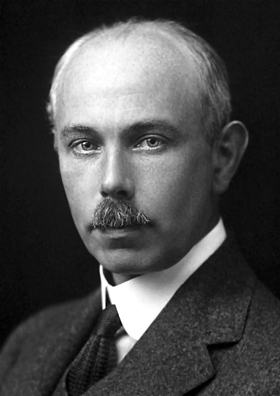
\includegraphics[width=\linewidth]{images/book3/aston.jpg}
\end{minipage}\hspace{0.02\linewidth}%
\begin{minipage}[t]{0.24\linewidth}
\vspace{0pt}
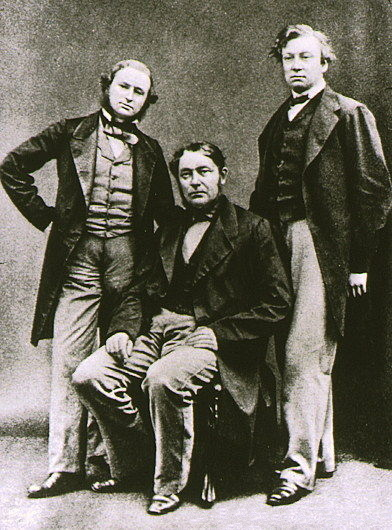
\includegraphics[width=\linewidth]{images/book3/kirchhoff-bunsen.jpg}
\end{minipage}\hfill
\begin{minipage}[t]{0.54\linewidth}
\vspace{0pt}
Gustav Kirchhoff y Robert Bunsen mostraron hacia 1860 que cada elemento da sus propias rayas en una llama,
y descubrieron el cesio y el rubidio por sus rayas desconocidas. El espectrógrafo de masas de Francis Aston, a partir de
1919, mostró que la mayoría de los elementos son mezclas de isótopos; recibió el Premio Nobel de Química de 1922.
(Fotografías: Aston, autor desconocido, dominio público; Kirchhoff, Bunsen y Henry Roscoe en 1862, de la
colección de Roscoe, dominio público; Wikimedia Commons.)
\end{minipage}
\end{history}

\section{Ejercicios}

\begin{exercise}[$\star$]\label{exo:b2:mass-spec-atomic:1}
Dese la $m/z$ de: el \omterm{def:b2:mass-spec-atomic:molecular-ion}{ion molecular} del benceno \ce{C6H6}; un ion de masa \qty{400}{u} con dos
cargas; la molécula protonada de la cafeína (\ce{C8H10N4O2}, masa nominal 194) formada por electrospray.
\end{exercise}

\begin{exercise}[$\star$]\label{exo:b2:mass-spec-atomic:2}
Un compuesto de C, H, N y O tiene un \omterm{def:b2:mass-spec-atomic:molecular-ion}{ion molecular} en $m/z$ 73. ¿Qué puede decirse de sus átomos de nitrógeno?
Propóngase una fórmula.
\end{exercise}

\begin{exercise}[$\star$]\label{exo:b2:mass-spec-atomic:3}
Un grupo de \omterm{def:b2:mass-spec-atomic:molecular-ion}{ion molecular} muestra dos picos separados dos unidades, de altura casi igual. Otro muestra dos
picos separados dos unidades en la razón 3 : 1. ¿Qué halógenos?
\end{exercise}

\begin{exercise}[$\star$]\label{exo:b2:mass-spec-atomic:4}
Una sal colorea una llama de amarillo; otra, de carmesí. Identifíquense los elementos y dense las longitudes de onda de sus
rayas.
\end{exercise}

\begin{exercise}[$\star\star$]\label{exo:b2:mass-spec-atomic:5}
Un hidrocarburo tiene $M$ al 100 \% y $M+1$ al 6.7 \%. ¿Cuántos átomos de carbono contiene?
\end{exercise}

\begin{exercise}[$\star\star$]\label{exo:b2:mass-spec-atomic:6}
Calcúlense las masas exactas de \ce{CO}, \ce{N2} y \ce{C2H4} y el poder de resolución necesario para separar
cada pareja.
\end{exercise}

\begin{exercise}[$\star\star$]\label{exo:b2:mass-spec-atomic:7}
El espectro IE de la pentan-3-ona muestra picos en 86, 57 (\omterm{def:b2:mass-spec-atomic:spectrum}{pico base}) y 29. Asígnense.
\end{exercise}

\begin{exercise}[$\star\star$]\label{exo:b2:mass-spec-atomic:8}
El espectro de la pentan-2-ona muestra picos en 86, 71, 58 y 43 (\omterm{def:b2:mass-spec-atomic:spectrum}{pico base}). Asígnense, y explíquese
por qué la pentan-3-ona solo muestra un pequeño pico en 58.
\end{exercise}

\begin{exercise}[$\star\star$]\label{exo:b2:mass-spec-atomic:9}
Patrones de cobre a 1.0, 2.0, 3.0 y \qty{4.0}{mg/L} dan absorbancias de 0.052, 0.104, 0.155 y 0.207;
una muestra da 0.128 (datos de ejercicio). Calcúlese su concentración de cobre.
\end{exercise}

\begin{exercise}[$\star\star\star$]\label{exo:b2:mass-spec-atomic:10}
En un analizador de tiempo de vuelo, $L = \qty{1.00}{m}$ y $U = \qty{20.0}{kV}$. Calcúlese el tiempo de vuelo de
un ion con una sola carga de masa \qty{1000}{u}, y el tiempo que lo separa de un ion de \qty{1001}{u}.
\end{exercise}

\begin{exercise}[$\star\star\star$]\label{exo:b2:mass-spec-atomic:11}
Calcúlese el grupo de \omterm{def:b2:mass-spec-atomic:molecular-ion}{ion molecular} del diclorometano, \ce{CH2Cl2}: valores de $m/z$ e intensidades
relativas.
\end{exercise}

\begin{exercise}[$\star\star\star$]\label{exo:b2:mass-spec-atomic:12}
En ICP-MS, el \ce{^{40}Ar^{16}O+} interfiere con el \ce{^{56}Fe+}. Calcúlese el poder de resolución necesario para
separarlos, y propóngase otra salida.
\end{exercise}

\section{Problema: un haluro desconocido}

\begin{problem}[{Problema de fin de semana --- un grupo de ion molecular con cloro y bromo, el número de
carbonos, los fragmentos, y una estructura contrastada con cada pico}]
\label{pb:b2:mass-spec-atomic:1}
Un líquido incoloro, eluido como un solo pico en \omterm{def:b2:chromatography:techniques}{cromatografía de gases}, da el \omterm{def:b2:mass-spec-atomic:spectrum}{espectro de masas} IE siguiente (datos del NIST
WebBook). Picos principales ($m/z$: intensidad relativa): 156: 14.5; 157: 0.5; 158: 18.6; 159: 0.6; 160:
4.4; 107: 6.7; 109: 6.3; 93: 3.3; 95: 2.9; 77: 59; 79: 18.7; 76: 39.5; 49: 12.9; 51: 4.3; 41: 100; 39:
26.2; 27: 24.6. Abundancias isotópicas: \ce{^{35}Cl} 0.758, \ce{^{37}Cl} 0.242, \ce{^{79}Br} 0.5069,
\ce{^{81}Br} 0.4931, \ce{^{12}C} 0.989, \ce{^{13}C} 0.011.
% ledger: ms:bromochloropropane, iso:Cl35, iso:Cl37, iso:Br79, iso:Br81, iso:C12, iso:C13, mass:C12, mass:H1, mass:Br79, mass:Cl35

\begin{center}
\begin{tikzpicture}
\begin{axis}[width=0.8\linewidth, height=4.6cm, xmin=20, xmax=170, ymin=0, ymax=112,
  xlabel={$m/z$}, ylabel={intensidad relativa}, label style={font=\small},
  tick label style={font=\scriptsize}, ycomb, xtick={27,41,49,77,93,107,122,156}]
\addplot[omDef, thick] table[x=mz, y=I] {figdata/out/bachelor-2-mass-spectra-d.dat};
\end{axis}
\end{tikzpicture}
\end{center}
% figdata: bachelor-2/mass-spectra.py part d

\medskip
\noindent\textbf{Parte I --- El \omterm{def:b2:mass-spec-atomic:molecular-ion}{ion molecular}.}
\begin{enumerate}
  \item ¿Qué picos forman el grupo del \omterm{def:b2:mass-spec-atomic:molecular-ion}{ion molecular}? ¿Por qué no es un solo pico?
  \item ¿Qué halógenos sugiere un grupo de tres picos separados 2 unidades?
  \item ¿Cuál es la masa nominal de la forma isotópica más ligera?
  \item ¿Qué dice la \omterm{def:b2:mass-spec-atomic:nitrogen-rule}{regla del nitrógeno}?
  \item Réstense un \ce{^{79}Br} y un \ce{^{35}Cl}: ¿qué queda, y qué fragmento hidrocarbonado
        tiene esa masa?
  \item Propóngase una fórmula molecular y dese su grado de insaturación.
\end{enumerate}

\medskip
\noindent\textbf{Parte II --- Carbonos y masa exacta.}
\begin{enumerate}[resume]
  \item A partir de la razón 157/156, estímese el número de carbonos.
  \item ¿Por qué es aquí tosca esa estimación?
  \item ¿Qué formas isotópicas contribuyen al pico en 158?
  \item Calcúlese la \omterm{def:b2:mass-spec-atomic:exact-mass}{masa monoisotópica} del \omterm{def:b2:mass-spec-atomic:molecular-ion}{ion molecular}.
  \item \ce{C10H20O} tiene también masa nominal 156 (exacta 156.151). ¿Qué poder de resolución separa
        ambos?
  \item ¿Tendría una masa nominal distinta el \omterm{def:b2:mass-spec-atomic:molecular-ion}{ion molecular} de un compuesto con un enlace C=C y los mismos halógenos?
\end{enumerate}

\medskip
\noindent\textbf{Parte III --- Fragmentos.}
\begin{enumerate}[resume]
  \item El par 77/79 está en la razón 3 : 1. ¿Qué átomo se ha perdido, y cuál es el ion?
  \item Explíquese el pico en 76.
  \item Asígnese el \omterm{def:b2:mass-spec-atomic:spectrum}{pico base} en 41.
  \item Asígnese el par 49/51.
  \item Asígnense los pares 93/95 y 107/109.
  \item ¿Por qué se pierde un átomo de bromo más fácilmente que un átomo de cloro?
  \item El 1-bromo-1-cloropropano daría \ce{CHBrCl+} en 127, 129 y 131. ¿Lo respalda el
        espectro?
\end{enumerate}

\medskip
\noindent\textbf{Parte IV --- La estructura.}
\begin{enumerate}[resume]
  \item Propóngase la estructura.
  \item Compruébese que explica cada pico de la lista.
  \item ¿Puede producirse una \omterm{def:b2:mass-spec-atomic:fragmentation}{transposición de McLafferty}? ¿Por qué?
  \item Dibújese el isómero que daría un pico intenso en $m/z$ 63/65 y ninguno en 49/51.
  \item ¿Qué formas isotópicas forman el pico en 160?
  \item A partir de las abundancias isotópicas, calcúlese la razón de los picos $M$, $M+2$ y $M+4$ para un
        cloro y un bromo, y compárese con el espectro.
\end{enumerate}
\end{problem}
